\documentclass[11pt]{article}
\usepackage[utf8]{inputenc}
\usepackage[T1]{fontenc}
\usepackage{amsmath,amssymb,booktabs,geometry,enumitem,graphicx,hyperref}
\geometry{margin=1in}

\newcommand{\norm}[1]{\left\|#1\right\|_2}
\newcommand{\Drill}{\mathrm{Drill}}
\newcommand{\Tail}{\mathrm{Tail}}
\newcommand{\CV}{\mathrm{CV}}

\title{\textbf{Graph Local Localization Algorithm}\\
\large merchant $\to$ user $\to$ order (MMD / cmean Drill) $\to$ one FSDS\\
\large (Non-causal; figure walkthrough)}
\author{TencentGR summary}
\date{2026-09-21}

\begin{document}
\maketitle

\begin{abstract}
We elaborate the \textbf{graph local localization} procedure behind the
four-panel figure
\texttt{three\_step\_subset\_localize.png}: standardize on $W_1$, rank
merchants then users by RBF-MMD$^2$, score orders by
$\|x-\mu_{\mathrm{user}}\|_2$, then run \textbf{one} FSDS on the
localized support. Objects $(\delta,D,r,\Tail,\CV,R)$ and the Drill
product rule decide early stop. No ATE claim.
\end{abstract}

\section{What is being localized}
TencentGR edge $=(u,i,t)$; terminal success $=$ click.
Merchant id $=$ \texttt{item\_feat.122} (encrypted shop proxy;
unmapped item $\to$ singleton shop).
Target $=$ period distribution shift $P^{W_1}$ vs $P^{W_2}$ on an
entity subset---not $\tau(S)$.
Graph only supplies nested keys; same procedure is modality-agnostic.

\begin{center}
\begin{tabular}{llll}
\toprule
layer & entity & score & panel \\
\midrule
L1 & merchant & RBF-MMD$^2(W_1,W_2)$ & top-left \\
L2 & user in $K_m$ & RBF-MMD$^2$ & top-right \\
L3 & order in $K_u$ & $\|x-\mu_u^{W_1}\|_2$ & bottom-left \\
stop & tip features & FSDS $F$-score & bottom-right \\
\bottomrule
\end{tabular}
\end{center}

\begin{figure}[h]
\centering
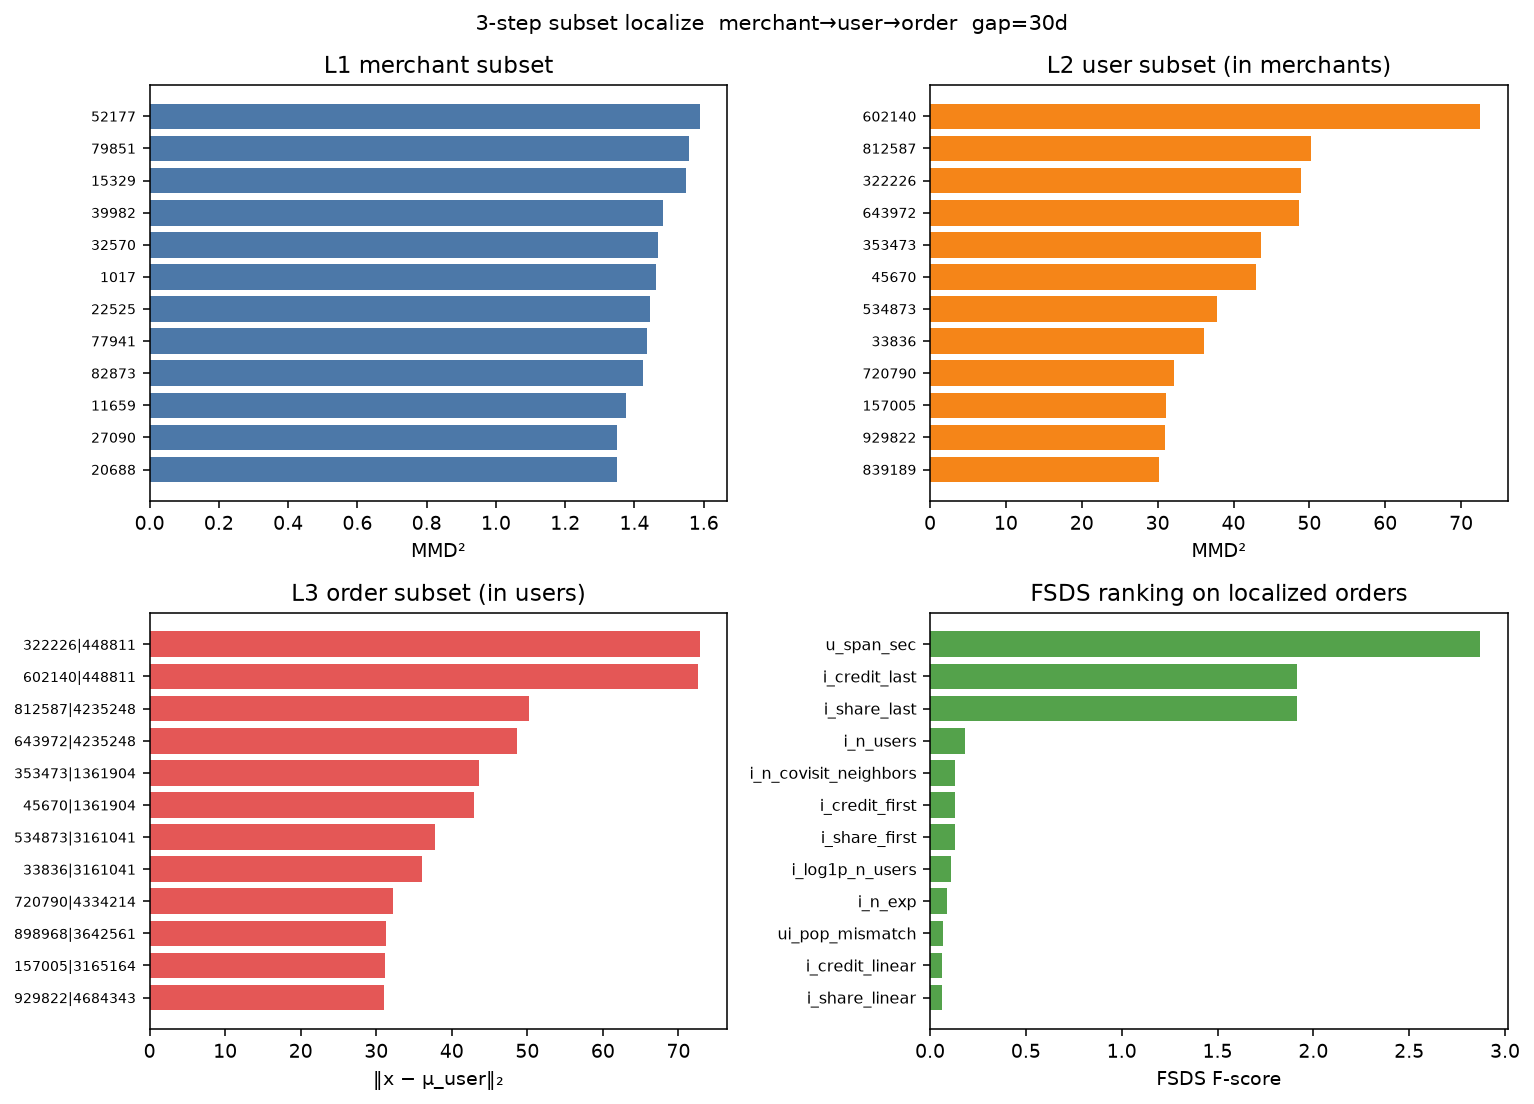
\includegraphics[width=0.95\textwidth]{three_step_subset_localize.png}
\caption{Prototype four-panel localize (gap $=30$d).}
\end{figure}

\section{Shared objects}
Parent support $S$, next key $v$:
\begin{align}
  \delta(S)&=\mu_S^{(W_2)}-\mu_S^{(W_1)},\\
  D_{v:}&=\mu_v^{(W_2)}-\mu_v^{(W_1)},
  \qquad r_v=\norm{D_{v:}},\\
  a_v&=\frac{\langle D_{v:},\delta\rangle}
            {\norm{D_{v:}}\,\norm{\delta}+\varepsilon}.
\end{align}
Spectrum: $\Tail(r)=$ Top-$K$ mass share;
$\CV(r)=\mathrm{sd}(r)/(\mathrm{mean}(r)+\varepsilon)$.
Residual of tip $K$:
$R(K)=\norm{\delta(S\setminus K)}^2/(\norm{\delta(S)}^2+\varepsilon)$.
In code, L1/L2 use MMD$^2$ (full-distribution) in place of $\|D\|_2$;
L3 uses $\ell_2$ to the user-$W_1$ mean (edge mass too thin for MMD).

\section{Four steps (reading the figure)}

\paragraph{Step 0 --- Standardization.}
Windowed FE; candidate columns (drop ranks / leakage).
\texttt{StandardScaler} fit on $W_1$ only; shared transform.

\paragraph{Step 1 --- L1 merchant (blue).}
For each candidate $m$ with $\ge n_{\min}$ edges in both windows
(volume-truncated):
\[
  \mathrm{score}(m)
  =\widehat{\mathrm{MMD}}^2(X_m^{W_1},X_m^{W_2})
  \quad\text{(RBF, median bandwidth, unbiased)}.
\]
Keep Top-$k_m\to K_m$; restrict edges.
\emph{Figure:} MMD$^2\approx 1.35$--$1.59$, relatively flat---several
merchants co-drift. Theory may D-stop here; default nest continues to
user for ops readability.

\paragraph{Step 2 --- L2 user (orange), inside $K_m$.}
Same MMD$^2$ on users; Top-$k_u\to K_u$.
\emph{Figure:} scores jump to $30$--$70$, sharp spectrum---canonical
\textbf{D-drill}: defer FSDS; shrink support.
Fallback: mean-shift $\| \mu_2-\mu_1\|$; then volume Top-$k$.

\paragraph{Step 3 --- L3 order (red), inside $K_u$.}
Order $=\texttt{user\_item\_ts}$ on terminal-success (else all edges).
Prefer $W_2$ rows; score $\|x-\mu_u^{W_1}\|_2$ in standardized space.
Top-$k_o$ for viz; FSDS mass uses merchant$\times$user edges.
\emph{Figure:} top orders co-locate with top users
(\texttt{322226|448811}, \texttt{602140|448811})---L3 names the
transaction tip of L2, not a new story.

\paragraph{Step 4 --- One FSDS (green).}
On final $K^\star$ (practice $=$ L2 user edges):
\[
  \mathrm{Scaler}\to\mathrm{Var}\to\mathrm{SelectKBest}(F)
  \to\mathrm{HGB}/\mathrm{LogReg},
\]
selection on $W_1$-train only; $W_2$ temporal holdout.
\emph{Figure:} tips
\texttt{u\_span\_sec}, \texttt{i\_credit\_last}, \texttt{i\_share\_last}.

\section{Drill product (early stop)}
\begin{equation}
  \Drill
  =
  \mathbf{1}\{\norm{\delta}\ge\varepsilon_\delta\}
  \cdot
  \mathbf{1}\{\Tail(r)\ge\tau\lor\CV(r)\ge c^\star\}
  \cdot
  \mathbf{1}\{R(K)\le R^\star\}
  \cdot
  \mathbf{1}\{\mathrm{mass}/\pi\ \mathrm{ok}\}.
\end{equation}
\begin{center}
\begin{tabular}{lll}
\toprule
$\|\delta\|$ & $r$ & action \\
\midrule
small & flat & Stop: no FSDS, no drill \\
large & flat & \textbf{Stop drill}; one FSDS on this layer \\
large & sharp & \textbf{Drill} to $K$; FSDS after $K^\star$ \\
sharp, $R\approx 1$ & --- & false tip $\to$ FSDS on $S$ \\
\bottomrule
\end{tabular}
\end{center}
\textbf{Column gates never license drill.} Nested keys:
merchant $\to$ user $\to$ order; evaluate Drill each layer;
when $\Drill=0$ or business cap binds, fix $K^\star$ and run
\textbf{exactly one} FSDS.

\section{Signed direction (required)}
After $K^\star$:
$\Delta\bar y=\bar y_{W_2}-\bar y_{W_1}$ (正向/负向/flat);
$\mathrm{sign}(\delta_j)$ on tips;
$s_v=\langle D_{v:},\delta\rangle$ for entity co-direction.
Forbidden: Top merchants/users without 正向/负向.

\section{Prototype numbers (gap $=30$d)}
$k_m{=}80$, $k_u{=}47$, $k_o{=}52$;
localized edges W1 $=324$, W2 $=6743$;
mapped\_rate $\approx 0.10$.
Reading: L1 spreads merchant candidates $\to$ L2 concentrates mass on
few users $\to$ L3 pins extreme orders $\to$ FSDS speaks only on the
narrowed support.

\paragraph{Mnemonic.}
Column-sharp + row-flat $=$ feature story (stop drill, FSDS).
Row-sharp $=$ entity story (drill).
FSDS hangs on the \emph{final} support only.

\section{CLI / sources}
\begin{verbatim}
PYTHONPATH=. python3 scripts/tencent_gr/run_three_step_subset_localize.py \
  --root data/tencent_subset --max-users 20000 --gap-days 30
\end{verbatim}
\texttt{docs/tencent\_gr/W1W2\_MMD\_PO\_LOCALIZE\_FSDS.md};
\texttt{docs/summaries/Graph\_Localize\_Algorithm\_Elaboration.md}.

\end{document}
